\documentclass[12pt]{article}
\usepackage{amsmath, amssymb}
\usepackage{geometry}
\usepackage{enumitem}
\usepackage{tikz}
\usetikzlibrary{automata, positioning, arrows.meta}

\geometry{margin=1in}

\title{\textbf{Theory of Computation --- Homework Solutions}\\
\large Chapter 0 (p.\ 25) \& Chapter 1 (p.\ 83)}
\author{}
\date{}

\begin{document}
\maketitle

%=============================================================
\section*{Chapter 0 Exercises}
%=============================================================

%-------------------------------------------------------------
\subsection*{Exercise 0.2 --- Formal Set Descriptions}
%-------------------------------------------------------------

\begin{enumerate}[label=(\alph*), start=2]

\item
\[
  \{ n \in \mathbb{Z} \mid n > 5 \}
\]

\item
\[
  \{ n \in \mathbb{N} \mid n < 5 \}
\]

\end{enumerate}

%-------------------------------------------------------------
\subsection*{Exercise 0.3 --- Set Operations}
%-------------------------------------------------------------

Let $A = \{x, y, z\}$ and $B = \{x, y\}$.

\begin{enumerate}[label=(\alph*)]

\item \textbf{Is $A \subseteq B$?}\\
No. 
\item \textbf{Is $B \subseteq A$?}\\
Yes. 
\item \[
  A \cup B = \{x,\, y,\, z\}
\]

\item \[
  A \cap B = \{x,\, y\}
\]

\item \[
  A \times B = \{(x,x),\,(x,y),\,(y,x),\,(y,y),\,(z,x),\,(z,y)\}
\]

\item \textbf{Power set of $B$}\\
\[
  \mathcal{P}(B) = \bigl\{\emptyset,\,\{x\},\,\{y\},\,\{x,y\}\bigr\}
\]

\end{enumerate}

%-------------------------------------------------------------
\subsection*{Exercise 0.4 --- Size of a Cartesian Product}
%-------------------------------------------------------------

If $|A|=a$ and $|B|=b$, then $|A \times B| = a \cdot b$.

\medskip
\textbf{Explanation.} An element of $A\times B$ is an ordered pair $(a_i, b_j)$.
For each of the $a$ choices of the first component there are $b$ independent choices for
the second component, giving $a \cdot b$ pairs in total.

%-------------------------------------------------------------
\subsection*{Exercise 0.5 --- Size of a Power Set}
%-------------------------------------------------------------

If $|C| = c$, then $|\mathcal{P}(C)| = 2^c$.

\medskip
\textbf{Explanation.} To form a subset of $C$, we decide independently for each of the
$c$ elements whether to \emph{include} it or \emph{exclude} it --- two choices per element.
By the multiplication principle there are $\underbrace{2 \times 2 \times \cdots \times 2}_{c} = 2^c$ subsets.

%=============================================================
\newpage
\section*{Chapter 1 Exercises}
%=============================================================

%-------------------------------------------------------------
\subsection*{Exercise 1.2 --- Formal Description of $M_1$}
%-------------------------------------------------------------

\[
  M_1 = (Q,\,\Sigma,\,\delta,\,q_1,\,F)
\]
where
\begin{align*}
  Q      &= \{q_1,\, q_2,\, q_3\},\\
  \Sigma &= \{a,\, b\},\\
  q_1    &\text{ is the start state},\\
  F      &= \{q_2\}.
\end{align*}

The transition function $\delta$ is:

\begin{center}
\begin{tabular}{c|cc}
       & \textbf{b} & \textbf{a} \\\hline
$q_1$  & $q_1$      & $q_2$      \\
$q_2$  & $q_3$      & $q_3$      \\
$q_3$  & $q_1$      & $q_2$      \\
\end{tabular}
\end{center}


%-------------------------------------------------------------
\subsection*{Exercise 1.3 --- State Diagram of $M$}
%-------------------------------------------------------------

\begin{center}
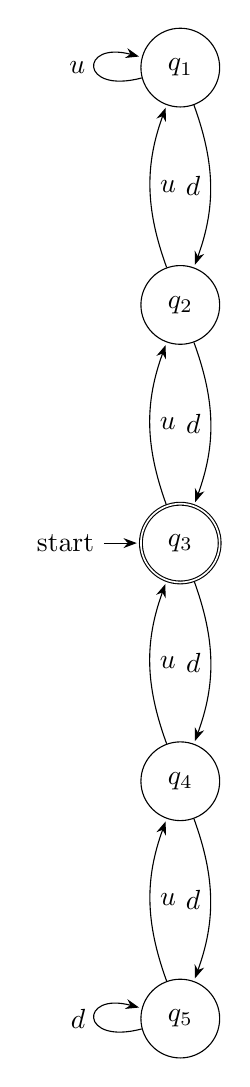
\begin{tikzpicture}[
    node distance=2cm,
    every state/.style={circle, draw, minimum size=1cm},
    >=Stealth,
    shorten >=1pt,
    auto
  ]

  \node[state]             (q1) {$q_1$};
  \node[state, below=of q1](q2) {$q_2$};
  \node[state, accepting, initial, below=of q2] (q3) {$q_3$};
  \node[state, below=of q3](q4) {$q_4$};
  \node[state, below=of q4](q5) {$q_5$};

  % u transitions (going up)
  \draw[->] (q2) edge[bend left=20]  node[right]{$u$} (q1);
  \draw[->] (q3) edge[bend left=20]  node[right]{$u$} (q2);
  \draw[->] (q4) edge[bend left=20]  node[right]{$u$} (q3);
  \draw[->] (q5) edge[bend left=20]  node[right]{$u$} (q4);

  % d transitions (going down)
  \draw[->] (q1) edge[bend left=20]  node[left]{$d$}  (q2);
  \draw[->] (q2) edge[bend left=20]  node[left]{$d$}  (q3);
  \draw[->] (q3) edge[bend left=20]  node[left]{$d$}  (q4);
  \draw[->] (q4) edge[bend left=20]  node[left]{$d$}  (q5);

  % self-loops
  \draw[->] (q1) edge[loop left]     node{$u$}        (q1);
  \draw[->] (q5) edge[loop left]     node{$d$}        (q5);

\end{tikzpicture}
\end{center}


%-------------------------------------------------------------
\subsection*{Exercise 1.36 --- $B_n = \{a^k \mid \text{where}\ k\ \text{is a multiple of}\ n\}$ is Regular}
%-------------------------------------------------------------

Build a DFA $D_n$ such that:
\[D_n=(\{q_0, q_1, \ldots, q_{n-1}\},\{a\},\delta,q_0,\{q_0\})\]
where for $\delta$, reading $a$ in state $q_i$ goes to state $q_{(i+1)\bmod n}$.\\\\
After reading $a^k$, the machine is in state $q_{k \bmod n}$.
It accepts if $k \bmod n = 0$.
Since $D_n$ is a DFA that recognizes $B_n$, the language $B_n$ is regular for every $n \ge 1$. 

%-------------------------------------------------------------
\subsection*{Exercise 1.37 --- $C_n = \{x \mid x \text{ is a binary multiple of } n\}$ is Regular}
%-------------------------------------------------------------
I asked AI for this question because I don't know what's a binary multiple.\\
Build a DFA $D_n$ such that:
\[D_n=(\{q_0, q_1, \ldots, q_{n-1}\},\{0,1\},\delta,q_0,\{q_0\})\]
For $\delta$, if the current state is $q_i$ \& the next bit is $b \in \{0,1\}$, then
        \[
          \delta(q_i,\, b) \;=\; q_{(2i + b)\bmod n}.
        \]
Why does this work: as you read the string left to right, each new bit $b$ transforms the current value $i$ into
$2i+b$.
\end{document}
